\documentclass[numeric]{fei}
\graphicspath{{images/}}
\usepackage{indentfirst}
\addbibresource{fontes.bib}

\begin{filecontents*}{\jobname.xmpdata}
\Title    {CARREGADOR WIRELESS POR LPT}
\Author   {Jagunço 1\sep Zé ninguem 2\sep Fulano 3}
\Copyright {Copyright \copyright\ 2020 "Douglas De Rizzo Meneghetti"}
\Keywords {manual\sep latex\sep tipografia}
\Language {pt-BR}
\Subject  {Resumo vai aqui em uma única linha corrida.}
\end{filecontents*}

% Preambulo
\title{CARREGADOR WIRELESS POR LPT}
\author{
	Gustavo Ryuji Sanomia\\
	Jaqueline Freitas Jardim\\
	Jéssica Trajano Matheus Benedito\\
	William Rodrigues Delmanto
}

\begin{document}
\maketitle

\begin{folhaderosto}
Dissertação de Mestrado apresentada ao Centro Universitárioda FEI para obtenção do título de Mestre em EngenhariaElétrica, orientado pelo Prof. Dr. Nome do Orientador.
\end{folhaderosto}

\fichacatalografica
\folhadeaprovacao

\dedicatoria{Essa é a dedicatoria}

\begin{agradecimentos}
A quem se deseja agradecer.
\end{agradecimentos}

\begin{resumo}
De tomada a bateria, de desktop a notebook, de telefone a celular, a palavra portabilidade vem ganhando cada vez mais força no cotidiano das pessoas. Sob essa perspectiva, a energia elétrica sem fio (wireless) chama cada vez mais atenção de pesquisadores e empresas ao redor do mundo, de modo a permitir ainda mais conforto no momento do carregamento destes dispositivos, sem a necessidade da utilização de cabos. O objetivo central do trabalho é abordar, analisar e desenvolver sobre o tema do carregador wireless, focando especialmente na tecnologia LPT (Laser Power Transmission), bem como o impacto desse modelo nos indivíduos, nas organizações e na sociedade como um todo. Propõe-se, assim, apresentar um produto transmissor e receptor de energia via LPT ressaltando suas limitações, diferenciações e singularidades deste método de carregamento a distância.
\palavraschave{\LaTeX{}. FEI.}
\end{resumo}

\begin{abstract}
From socket to battery, from desktop to notebook, from telephone to cellphone, the portability word has been gaining more strength in people's daily lives. From this perspective, wireless electricity draws even more attention from researchers and companies all around the world, in order to allow even more comfort when charging these devices, without the need to use cables. The main objective of this study is to approach, analyze and develop on the wireless charger topic, focusing especially on LPT technology (Laser Power Transmission), as well as the impact of this model on people, organizations and society as a whole. Therefore, the proposal is to present a product that transmits and receives energy via LPT emphasizing its limitations, differences and singularities of this distance charging method.
\keywords{\LaTeX{}. FEI.}
\end{abstract}

\listoffigures
\listoftables
%\printglossaries
\tableofcontents

\chapter{Introdução}

\section{Objetivo}

Compreender e aplicar o conceito da tecnologia LPT (Laser Power Transmission) a fim de desenvolver um dispositivo móvel capaz de transmitir energia sem fio, que seja compacto e seguro, para atender as mais diversas aplicações de baixo consumo energético, baseando-se em estudos já existentes.

\section{Justificativa}

Portabilidade tem sido uma das grandes evoluções da tecnologia nos últimos 30 anos, principalmente em relação à celulares e notebooks, e mais recentemente em relação a tablets. Seguindo a evolução dos telefones fixos para os celulares e dos computadores desktop para os notebooks de última geração de apenas 1kg, nota-se que mobilidade tornou-se uma característica chave de nossas tecnologias \cite{liu16}.  Quando os primeiros celulares chegaram ao Brasil em 1990 eram apenas 667, já em 2010 passaram a ser 197,53 milhões de aparelhos [2], para chegarem à marca de 230 milhões em 2020 [3]. Os novos celulares, tablets e notebooks têm sido lançados com baterias mais duráveis e com circuitos cada vez mais energeticamente eficientes; porém ainda é necessário o carregamento da bateria destes dispositivos uma vez por dia. Outro ponto a ser considerado é a degradação notória das baterias, geralmente celulares, notebooks e tablets são usados diariamente, porém com o passar do anos fica evidente a degradação de suas baterias [4].

Nota-se, também a grande tendência do mundo wireless (sem fio), a grande maioria das marcas já estão oferecendo fones bluetooth e celulares com carregadores indutivos, porém estes têm de estar perto de uma tomada. O próximo passo da portabilidade desses aparelhos está relacionado completamente à forma como vamos carregar suas baterias. Portanto, a tecnologia LPT mostra-se como uma possível solução de wireless charging para esta questão. No mercado já existe um produto de wireless charging da empresa israelita Wi-Charge, criada em 2012; seus produtos são focados para aplicações de baixo potência, como celulares, torneiras elétricas automáticas e aparelhos de smart home [5].

Há outras diversas aplicações como sensores autônomos, inclusive subaquáticos, cada vez mais usados para aplicações militares, de segurança de fronteiras, ciência e industriais, da exploração de petróleo à agricultura; veículos subaquáticos não tripulados, como aqueles usados para exploração de petróleo e inspeção de estruturas submarinas, onde o peso dos cabos de cobre impede significativamente sua utilidade; torres de retransmissão de telecomunicações geralmente estão localizadas longe de estradas e linhas de energia, e frequentemente em locais onde o clima, o terreno ou mesmo a aparência limitam o uso de painéis solares [6].

\chapter{Revisão bibliográfica}

\section{LASER}

Sinônimo de alta tecnologia e considerado uma das maiores invenções do século XX o Laser (Light Amplification by Stimulated Emission of Radiation) é um dispositivo que possibilita a amplificação da luz por emissão estimulada de radiação, essa característica o diferencia de fontes luminosas comuns proporcionando uma vasta gama de aplicações nas mais diversas áreas da indústria, medicina, militar, telecomunicações etc.

\subsection{Contexto histórico}

Em 1900, Max Planck, o "Pai da Física Quântica", descobriu que "A radiação é absorvida ou emitida por um corpo aquecido através de pequenos 'pacotes' de energia, não sob a forma de ondas. Esses "pacotes" denominados quantum são os fótons da energia eletromagnética que, segundo o físico dinamarquês Niels Bohr, é a quantidade de energia absorvida ou emitida pelo elétron nas suas transições de órbitas.

A compreensão de que a luz é uma forma de partícula foi fundamental para o estudo de Einstein sobre emissão estimulada apresentado no "The Quantum Theory of Radiation"(1917) que foi a primeira publicação sobre o conceito de radiação a laser.

A teoria de Albert Einstein diz que um átomo perturbado por um fóton que incide sobre ele, emite um outro fóton de mesma fase, frequência, polarização e direção do original, esse processo ocorre como efeito cascata. A luz é gerada somente quando os fótons emitidos forem maiores do que os absolvidos.

Quando a emissão ocorre espontaneamente, a energia é liberada de forma arbitrária e em diferentes frequências. Enquanto a emissão estimulada, por possuir maior coerência, o efeito amplifica a absorção da energia radioativa original.

Em uma época que a exploração do espectro magnético era limitada, um grupo de cientistas estadunidenses e russos: Charles Townes e Jim Gordon, e Nicolay Basov e Alexsander Prokhorov, desenvolveram separadamente em 1954, um dispositivo que amplifica as microondas, o MASER (Microwave Amplification by Stimulated Emission of Radiation), ou seja, amplificação de microondas pela emissão estimulada de radiação.

Utilizou-se a amônia como meio ativo. O funcionamento deste dispositivo ocorria ao ser excitado por um agente externo, a molécula de amônia entra em vibração com uma frequência de microondas, essa emissão estimulada gera um feixe coerente de microondas. Essa descoberta é considerada o precursor do laser, o que lhes concedeu o prêmio Nobel de Física em 1964.

O primeiro laser foi apresentado em 16 de maio de 1960, pelo físico estadunidense Theodore Maiman, sendo o cristal de rubi o meio ativo do dispositivo.

\begin{quote}
Uma fonte de luz, na forma do poderoso clarão de uma lâmpada, irradiou um cristal de rubi sintético [com duas faces paralelas cobertas de prata], que absorveu energia sobre uma ampla banda de frequências. Essa energia ótica excitou os átomos até um estado de maior energia, do qual a energia foi irradiada novamente em uma estreita banda de frequências. Os átomos excitados foram acoplados a um ressonador óptico e estimulados a emitir juntos a radiação. (T. H. Maiman Nature 187, 493–494; 1960).
\end{quote}

Nas décadas seguintes, este instrumento passou a ser cada vez mais presente no cotidiano e tornou-se fundamental nas mais diversas atividades, sendo utilizado em soldagens, impressoras, cirurgias, holografia, equipamentos de cirurgia dentária, leitores de CD e DVD, leitor de código de barra, ciência biomédica etc.

\subsection{Teoria}

\par
Segundo SEARS and ZEMANSKY (2016, p.255) sabe-se que o fóton é emitido quando um átomo em um estado excitado "cai" para um estado de energia inferior, sendo que esse estado dura alguns nanosegundos. Átomos e moléculas podem também absorver fótons, efetuando então uma transição de um nível energético inferior para um superior. Quanto mais alta a temperatura, maior a probabilidade de ocorrer colisões, sendo que estas provocam transições para níveis energéticos superiores.
Como foi mencionado no contexto histórico, Albert Einstein, baseando-se na mecânica quântica, teorizou o princípio do funcionamento do raio laser, a partir da emissão estimulada:

\begin{quote}
Se um átomo no estado excitado é iluminado por um fóton que tem a mesma energia da transição que ocorreria espontaneamente, o átomo pode ser estimulado a voltar ao estado de mais baixa energia e simultaneamente emitir um fóton com a mesma energia da transição e mesma direção do fóton incidente. Assim, um único fóton que interage com um átomo excitado pode resultar então em dois fótons. Se usarmos a descrição ondulatória da luz, a emissão estimulada terá a freqüência da luz incidente e estará em fase (coerente), resultando em amplificação da intensidade da onda de luz original. (Zilio, 2009, p.212).
\end{quote}

Segundo Zilio (2009, p.213) na ausência de colisões, as moléculas tendem a permanecer no estado energético mais baixo disponível. Ou seja, estados de energia alta são sempre menos povoados que o estado fundamental, sendo a absorção superior à emissão estimulada.

"A probabilidade da emissão estimulada é idêntica à probabilidade da absorção estimulada." (A. Einstein Phys. Z. 18, 121, 1917)

\begin{quote}
...como o número de átomos no estado excitado é muito pequeno com relação ao do estado fundamental, o fóton emitido tem uma probabilidade muito maior de ser re-absorvido, fazendo a emissão estimulada insignificante quando comparada com a emissão espontânea (no equilíbrio termodinâmico). O mecanismo pelo qual a emissão estimulada pode se tornar dominante é ter mais átomos no estado excitado que no estado fundamental, de forma que os fótons emitidos têm maior probabilidade de estimular a emissão do que serem absorvidos. Como esta condição é o inverso do que ocorre na situação de equilíbrio normal, ela é denominada de inversão de população. Havendo mais átomos num estado excitado que no fundamental, a emissão estimulada pode dominar, resultando numa cascata de fótons. O primeiro fóton emitido estimulará a emissão de mais fótons, que estimularão a emissão de ainda mais fótons, e assim por diante. A cascata resultante de fótons cresce, produzindo a amplificação da luz emitida. Se a inversão de população termina (a população do estado fundamental domina), a emissão espontânea se tornará novamente o processo favorecido.(Zilio, 2009, p.213)
\end{quote}

Para que a excitação do meio ativo ocorra é necessário utilizar uma fonte de excitação externa, ou seja, um mecanismo de bombeamento que varia conforme o meio escolhido, podendo ser lâmpadas flash, lâmpadas de arco, outro laser e etc.

No laser, a emissão de luz acontece somente quando o ganho supera as perdas, sendo que este ocorre quando há inversão de população, para que este fenômeno aconteça é necessário que os fótons fiquem confinados em uma cavidade ressonante, de forma a serem utilizados para desencadear mais processos de emissão estimulada, caso contrário, o sistema irradia para todas as direções.

A cavidade ressonante óptica é rodeada por dois espelhos, um parcialmente e o outro totalmente refletor, o que torna o processo de emissão estimulada maximizado, pois o feixe resultante é forçado a atravessar ciclicamente o meio ativo provocando o aumento da intensidade a cada volta completa (“round trip”). Além disso, esse processo faz com que a emissão ocorra em uma mesma fase, a propriedade de vibração em fase chama-se coerência espacial (RIBEIRO, 2000; SVELTO,2010).

Portanto, o dispositivo necessita satisfazer três condições fundamentais para operação:

\begin{itemize}
	\item Meio ativo: sólido, líquido ou gasoso;
	\item Mecanismo de excitação ou bombeamento;
	\item Ressonador ou cavidade ressonante.
\end{itemize}

As outras fontes luminosas são emitidas espontaneamente sem nenhuma intervenção externa apresentando ondas com diferentes comprimentos e frequência, de forma a viajar no espaço e tempo incoerentemente.

Monocromático: a radiação ocorre em um único movimento de onda ou cor, portanto possui um estreito intervalo de comprimento de onda. O quadro X mostra os comprimentos de onda para alguns tipos de laser.

\begin{quadro}
\centering
\caption{Principais comprimentos de onda de emissão de alguns lasers}
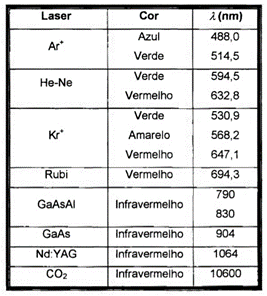
\includegraphics{tabela_laser}
\smallcaption{Fonte: Autor}
\end{quadro}

Brilho: grande intensidade de luz;

Direcionalidade: feixe propaga-se na mesma direção, havendo um mínimo de dispersão;

Coerência: onda de mesmo comprimento e fase.

\subsection{Propriedades}

As suas características proporcionam propriedades diferenciadas em relação às outras demais fontes de luz. Assim, Bagnato (2001, p.9) aponta os principais aspectos:

Monocromático: a radiação ocorre em um único movimento de onda ou cor, portanto possui um estreito intervalo de comprimento de onda. O quadro X mostra os comprimentos de onda para alguns tipos de laser.

\subsection{Feixe Gaussiano}

Em condições ideais, a luz de um laser assume a forma de um Feixe Gaussiano, ou seja, a luz pode ser transportada e confinada na forma de feixe, apresentando mínima divergência. (SALEH; TEICH, 1991, p.81)

As principais características deste tipo de feixe óptico são:

\begin{itemize}
	\item A concentração de potência do feixe encontra-se dentro de um cilindro que envolve o eixo do feixe.
	\item A distribuição de intensidade em qualquer plano transversal é uma função gaussiana circularmente simétrica centrada em torno do feixe.
	\item A largura desta função é mínima na cintura do feixe e tornando-se gradualmente maior à medida que as distâncias entre entre as cintura aumentam nos dois sentidos.
	\item As frentes de ondas são aproximadamente planar perto da cintura do feixe, gradualmente se curva com o aumento da distância para a cintura, e em última instância, torna-se aproximadamente esférica longe da cintura.
	\item A divergência angular das normais de frente de onda assume o valor mínimo permitido pela equação de onda para uma determinada largura de feixe. Sob condições ideais , a luz a partir de muitos tipos de laser toma a forma de um feixe de Gauss.
\end{itemize}

O modo gaussiano transversal fundamental (TEM00) é o mais usado na maioria das aplicações lasers, sendo a amplitude complexa do feixe Gaussiano expressa em U (X) (SALEH; TEICH, 1991, p.83).

\begin{equation}
\label{eq:gaussiano}
U_{(r)}=A_0\frac{W_0}{W_{(z)}}exp\left [ -jkz-jk\frac{\rho ^2}{2R_{(z))}}+j\zeta_{(z)} \right ]
\end{equation}

Onde $\rho$ é a distância radial ao eixo do feixe, $z$ distância axial a partir do foco do feixe, $k = 2\pi/\lambda$ (número de onda por comprimento de onda), $U$ amplitude do campo elétrico, $W$ raio do qual a amplitude tem decaimento de $1/e$, $W_{(0)}$ tamanho da cintura, $R$ raio de curvatura da frente de onda e a fase de Gouy.

Os cálculos (X), (X), (X) e (X) determinam as propriedades do feixe gaussiano (SALEH; TEICH, 1991, p.83). Nas equações são considerados os parâmetros $A_0$ e $Z_0$ determinados pelas condições de fronteira e   que é o comprimento de onda.

A Figura 1 apresenta as propriedades do feixe gaussiano.

\begin{figure}
\centering
\label{feixe_gaussiano}
\caption{Feixe gaussiano}
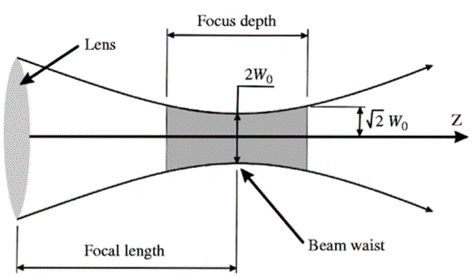
\includegraphics{feixe_gaussiano}
\smallcaption{Fonte: Autor}
\end{figure}

\subsubsection{Largura de feixe}

Dentro de qualquer plano transversal, a intensidade do feixe assume seu valor de pico no eixo, e tem um fator de decaimento = 0,135 na distância radial $\rho = W_{(z)}$, sendo 86\% da energia é transportada dentro de um círculo de raio W (z), consideramos W (z) como o feixe raio (também chamado de largura do feixe). A largura rms da distribuição de intensidade é $\sigma = 1/2W_{(z)}$. (SALEH; TEICH, 1991, p.85)

\begin{equation}
\label{eq:gaussiano_largura}
W_{(z)} = W_0 \left [ 1 + \left( \frac{z}{z_0} \right ) ^2 \right ] ^{1/2}
\end{equation}

Assume-se valor mínimo Wo no plano $z = 0$, denominado cintura do feixe. Assim Wo é o raio da cintura. O diâmetro da cintura $2W_0$ é chamado de tamanho do ponto. (SALEH; TEICH, 1991, p.85)

\begin{equation}
\label{eq:raio_cintura_1}
W_0 = \left( \frac{\lambda z_0}{\pi} \right)^{1/2}
\end{equation}

\begin{equation}
\label{eq:raio_cintura_2}
W_{(z)} = \frac{\lambda z_0}{\pi} z = \theta_0 z
\end{equation}

\begin{figure}
\centering
\label{beam_optics}
\caption{Optica do feixe}
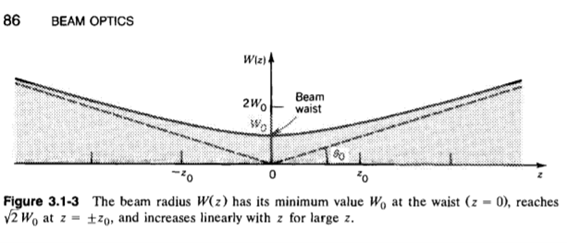
\includegraphics{beam_optics}
\smallcaption{Fonte: Autor}
\end{figure}

\subsubsection{Raio de curvatura}

\begin{equation}
\label{eq:raio_curvatura}
R_{(z)} = z \left [ 1 + \left( \frac{z_0}{z} \right ) ^2 \right ]
\end{equation}

\subsubsection{Fase de Gouy}

\begin{equation}
\label{eq:fase_gouy}
\zeta_{(z)} = tan^{-1} \frac{z}{z+0}
\end{equation}

Potência
A potência óptica total transportada no plano transversal. (SALEH; TEICH, 1991, p.85)

\begin{equation}
\label{eq:potencia}
P = \frac{1}{2}I_0(\pi W_0^2)
\end{equation}

Intensidade do eixo
A equação (X) quantifica a intensidade no centro do feixe em sua cintura:

\begin{equation}
\label{eq:intencidade_eixo}
I_0 = \frac{E_0^2}{2\eta}
\end{equation}

Sendo $\eta$ a impedância característica do meio, para o espaço livre, $\eta = \eta_0 = 377 \Omega$. Feixes ópticos são usualmente caracterizados pela potência $P$ então é útil escrever $I_0$ em temos de $P$ (SALEH; TEICH, 1991, p.85)

\cite{latexcompanion} \cite{einstein}

\printbibliography
%\printindex
\end{document}